\documentclass[english]{tktltiki}
\usepackage[pdftex]{graphicx}
\usepackage{subfigure}
\usepackage{url}
\begin{document}
%\doublespacing
%\singlespacing
\onehalfspacing

\title{Assignment 1: Improvement of the interaction of a website}
\author{P�ter Ivanics}
\date{\today}

\maketitle

\numberofpagesinformation{\numberofpages\ pages + \numberofappendixpages\ appendices}
\keywords{}

\mytableofcontents

\section{Introduction}
	This short report contains a heuristic evaluation and improvement of a simple one-page website. The report is rolled out as one of the assignment of the Human-Computer Interaction course and serves the purpose to gain hands-on experience with the course material. The given webpage of discussion is displayed on Figure \ref{original_webpage}. 
	
	\begin{figure}[h] 
		\begin{center}
			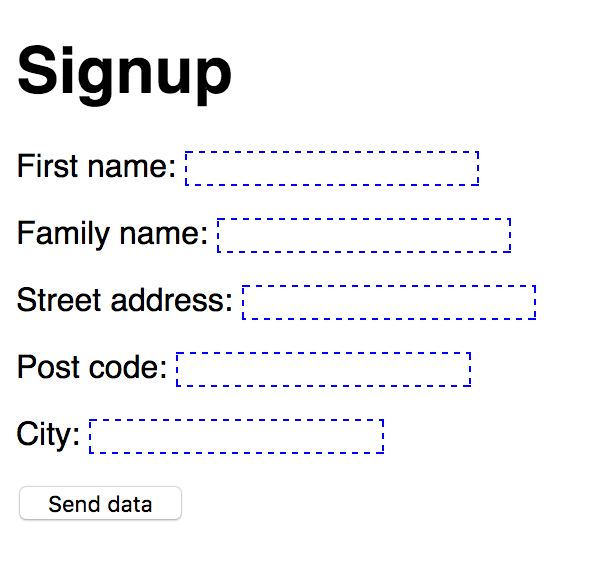
\includegraphics[height=0.4\textwidth]{images/original_webpage.png}
			\caption{The webpage of discussion in its original state, that is going to be analyzed and improved in this report.}
			\label{original_webpage}
		\end{center}
	\end{figure}

	As shown, the webpage includes a very simple web form with the purpose of user registration for a service .The page has a title of "Online shop -- Registration", a couple of labels and textboxes and a button in the bottom which is supposed to validate and submit the data if all fields are filled correctly by the user. The next chapter of this report describes the heuristic evaluation of the website, which means listing the proposed suggestions, improvement possibilities, design ideas and features for this simple form. The evaluation is mainly based on the course material and the contents of the book Don't Make me Think by Steve Krug \cite{SK14}. Further, a short description about the implementation is given which is based on the former evaluation. Finally, the last chapter concludes the report and describes further improvement possibilities for the website. 

\section{Heuristic evaluation}

% [description of the usability characteristics used, and UI improvements planned based on them]
	To set the context, the term of heuristic evaluation is defined shortly. As discussed on the lecture, heuristic evaluation is one of the possible methods for performing usability testing of a website or system. The heuristic method means performing the evaluation without end-user involvement. This is done on the given single page with the utilization of the discussed usability characteristics and explanation on User Centered Design (UCD) during the lecture.
	
	 To begin the analysis with, the original form displayed on Figure \ref{original_webpage} is as minimalistic as possible. In general this should not be considered as a problem, but rather as a possibility, because this observation gives a lot of room for improvements. Taking the first look at the original webpage, one can immediately see what it is about - the user is expected to provide certain information about him/herself to sign up for a service. Nevertheless, one notices soon that this page does not correspond to today's standards, the page is not optimized for mobile devices and usability can be greatly enhanced by applying some simple modifications. Due to the simplicity of the page, too many use-case scenarios cannot be investigated and therefore only the inspection of this screen is explained. The suggestions to follow are explained in importance order (from the most important to the least important). 
	 
	 The most important principle to point out during the improvement of a web page is the "Don't make me think" principle \cite{SK14}. To summarize in one sentence, the meaning is to keep the webpage as self-evident and obvious as possible. As suggestions are made for improving the look \& feel of the site, the aspects below should be kept in mind all the time. When a user is presented this page, they should immediately understand that 
	 
	\begin{enumerate}
		\item they are on a registration form, 
		\item what are they signing up for,
		\item what information are they required to give,
		\item how do they submit that information,
		\item what happens after the information is submitted/where the data is going to be go,
		\item what subset of the information is mandatory (i.e. which are the mandatory fields and which ones can be skipped).
	\end{enumerate}
	
	The next suggestion would be to ensure users will know how to use the form. Naturally, this strongly correlates with the previous "Don't make me think" principle \cite{SK14}. To be more specific, the form should have standard controls, use common conventions, metaphors and keep up the clarity and consistency. This would mean maintaining the same elements size of the elements on the screen, usage of the same colors, font size and type consistently. The content should be organized in a logical manner, for instance the items in the form should be in a reasonable order and the submit button should stay on the bottom of the form.
	
	To increase user attention and have a good first impression, the page could have some lively colors while keeping up an aesthetic and minimalistic design. This also means that the text should remain legible, the more important content should be emphasized using larger font size and there should be contrast between the text and the background's color. 
	
	Next up, as the user starts filling the form, he/she should get immediate feedback about the correctness of the information. For instance, when one of the textboxes looses focus, the borders of the control could turn green, if the given information is correct or red, if the entered value is invalid. This will give immediate feedback to the user about the input and help to avoid errors. An additional aim is to avoid potential errors as much as possible, for instance using dropdown selection for the city field rather than open text fields whenever possible \cite{SK14}. In case open text fields expect to have an input of a pre-defined format, the interface should intuitively help the user as suggested by Kim \cite{KIM15}. In case one of the values is incorrect, helpful error messages should indicate the cause of the problem and help the user to make proper corrections.
	
	Last but not least, to keep up to today's standards, the page should support mobile devices. Supporting multiple screen sizes and browsers would add value to the site and greatly enhance user experience along various platforms and therefore should be kept in mind during the implementation. Of course, in a real scenario this may not be necessary depending on the targeted audience, however it is good to be on the save side in this matter. Fortunately, there are many popular and ready-made solutions that provide wide support for all screen sizes. 
	
	\begin{table}[]
		\centering
		\caption{The most important usability aspects for the improvement of the webpage.}
		\label{usability_characteristics_table}
		\begin{tabular}{ll}
			Priority & Usability aspect                           \\
			1        & "Don't make me think" / being self-evident \\
			2        & Consistency and standards                  \\
			3        & Visibility and logical layout              \\
			4        & Aesthetic and minimalistic design          \\
			5        & Legibility and harmonized colors           \\
			6        & Feedback                                   \\
			7        & Error prevention and recovery              \\
			8        & Support for mobile                        
		\end{tabular}
	\end{table}		
	
	To summarize the suggestions in preference order, they are listed in Table  \ref{usability_characteristics_table} below. During the implementation these aspects are going to be kept in mind as indicated with their priority order. 
	
\section{Implementation}
	% [description that helps the lecturer(s) to understand your solution; does not need to be long]
	To begin with, a logo was added on the top of the screen so users understand which company's/brand's webpage they are browsing and what kind of service they are signing up for. Secondly, the labels from the textboxes were moved to placeholders to save some of the space and reduce the needless words on the screen.  The title was renamed to "Registration form" and the button's label was changed to "Submit". These indicate a bit more clearly what is happening on the page.
	
	\begin{figure}[h] 
		\begin{center}
			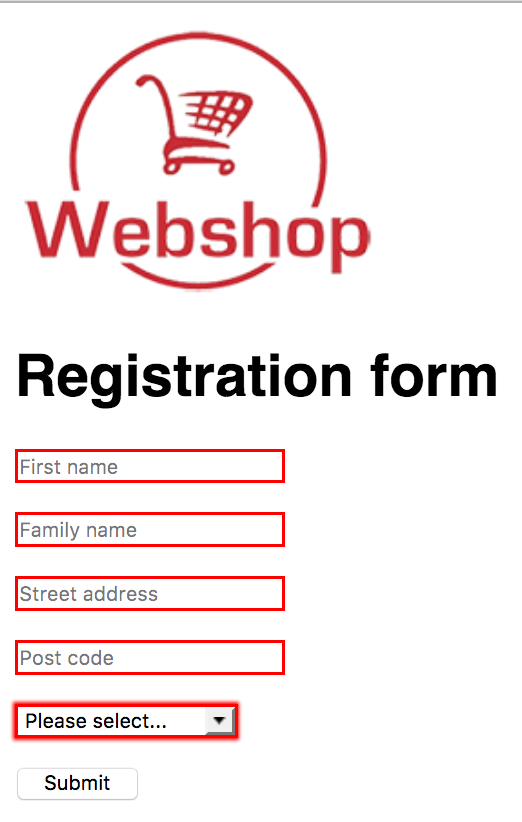
\includegraphics[height=0.4\textwidth]{images/webpage_halfway.png}
			\caption{The Webpage after small adjustments to the form.}
			\label{webpage_halfway}
		\end{center}
	\end{figure}
	
	Next, the city field was changed to a dropdown list. The items in the dropdown list are populated using the given $backendsimulator.getCities()$ function. This greatly enhances usability and avoids many potential errors. The street address input field was moved below the city. The reason behind this decision is the logical order of the fields. Finally, each field was made required. On top of that, the CSS settings were configured in a way that each field has a reddish border if the inserted values are invalid and green if the inserted values are valid. This gives immediate feedback to the users as they are typing so errors can be corrected accordingly. At this point of time, the page looked like as displayed on Figure \ref{webpage_halfway}. 
	
	Next, regular expressions were applied to ensure validation. Afterwards, Bootstrap was added to the page to support mobile devices and multiple screen sizes. At the same time, layout adjustments were made. Finally, colors were added to the CSS so the page became more attractive and lively. The final result is shown on Figure \ref{improved_webpage}. 
	
	\begin{figure}[h] 
		\begin{center}
			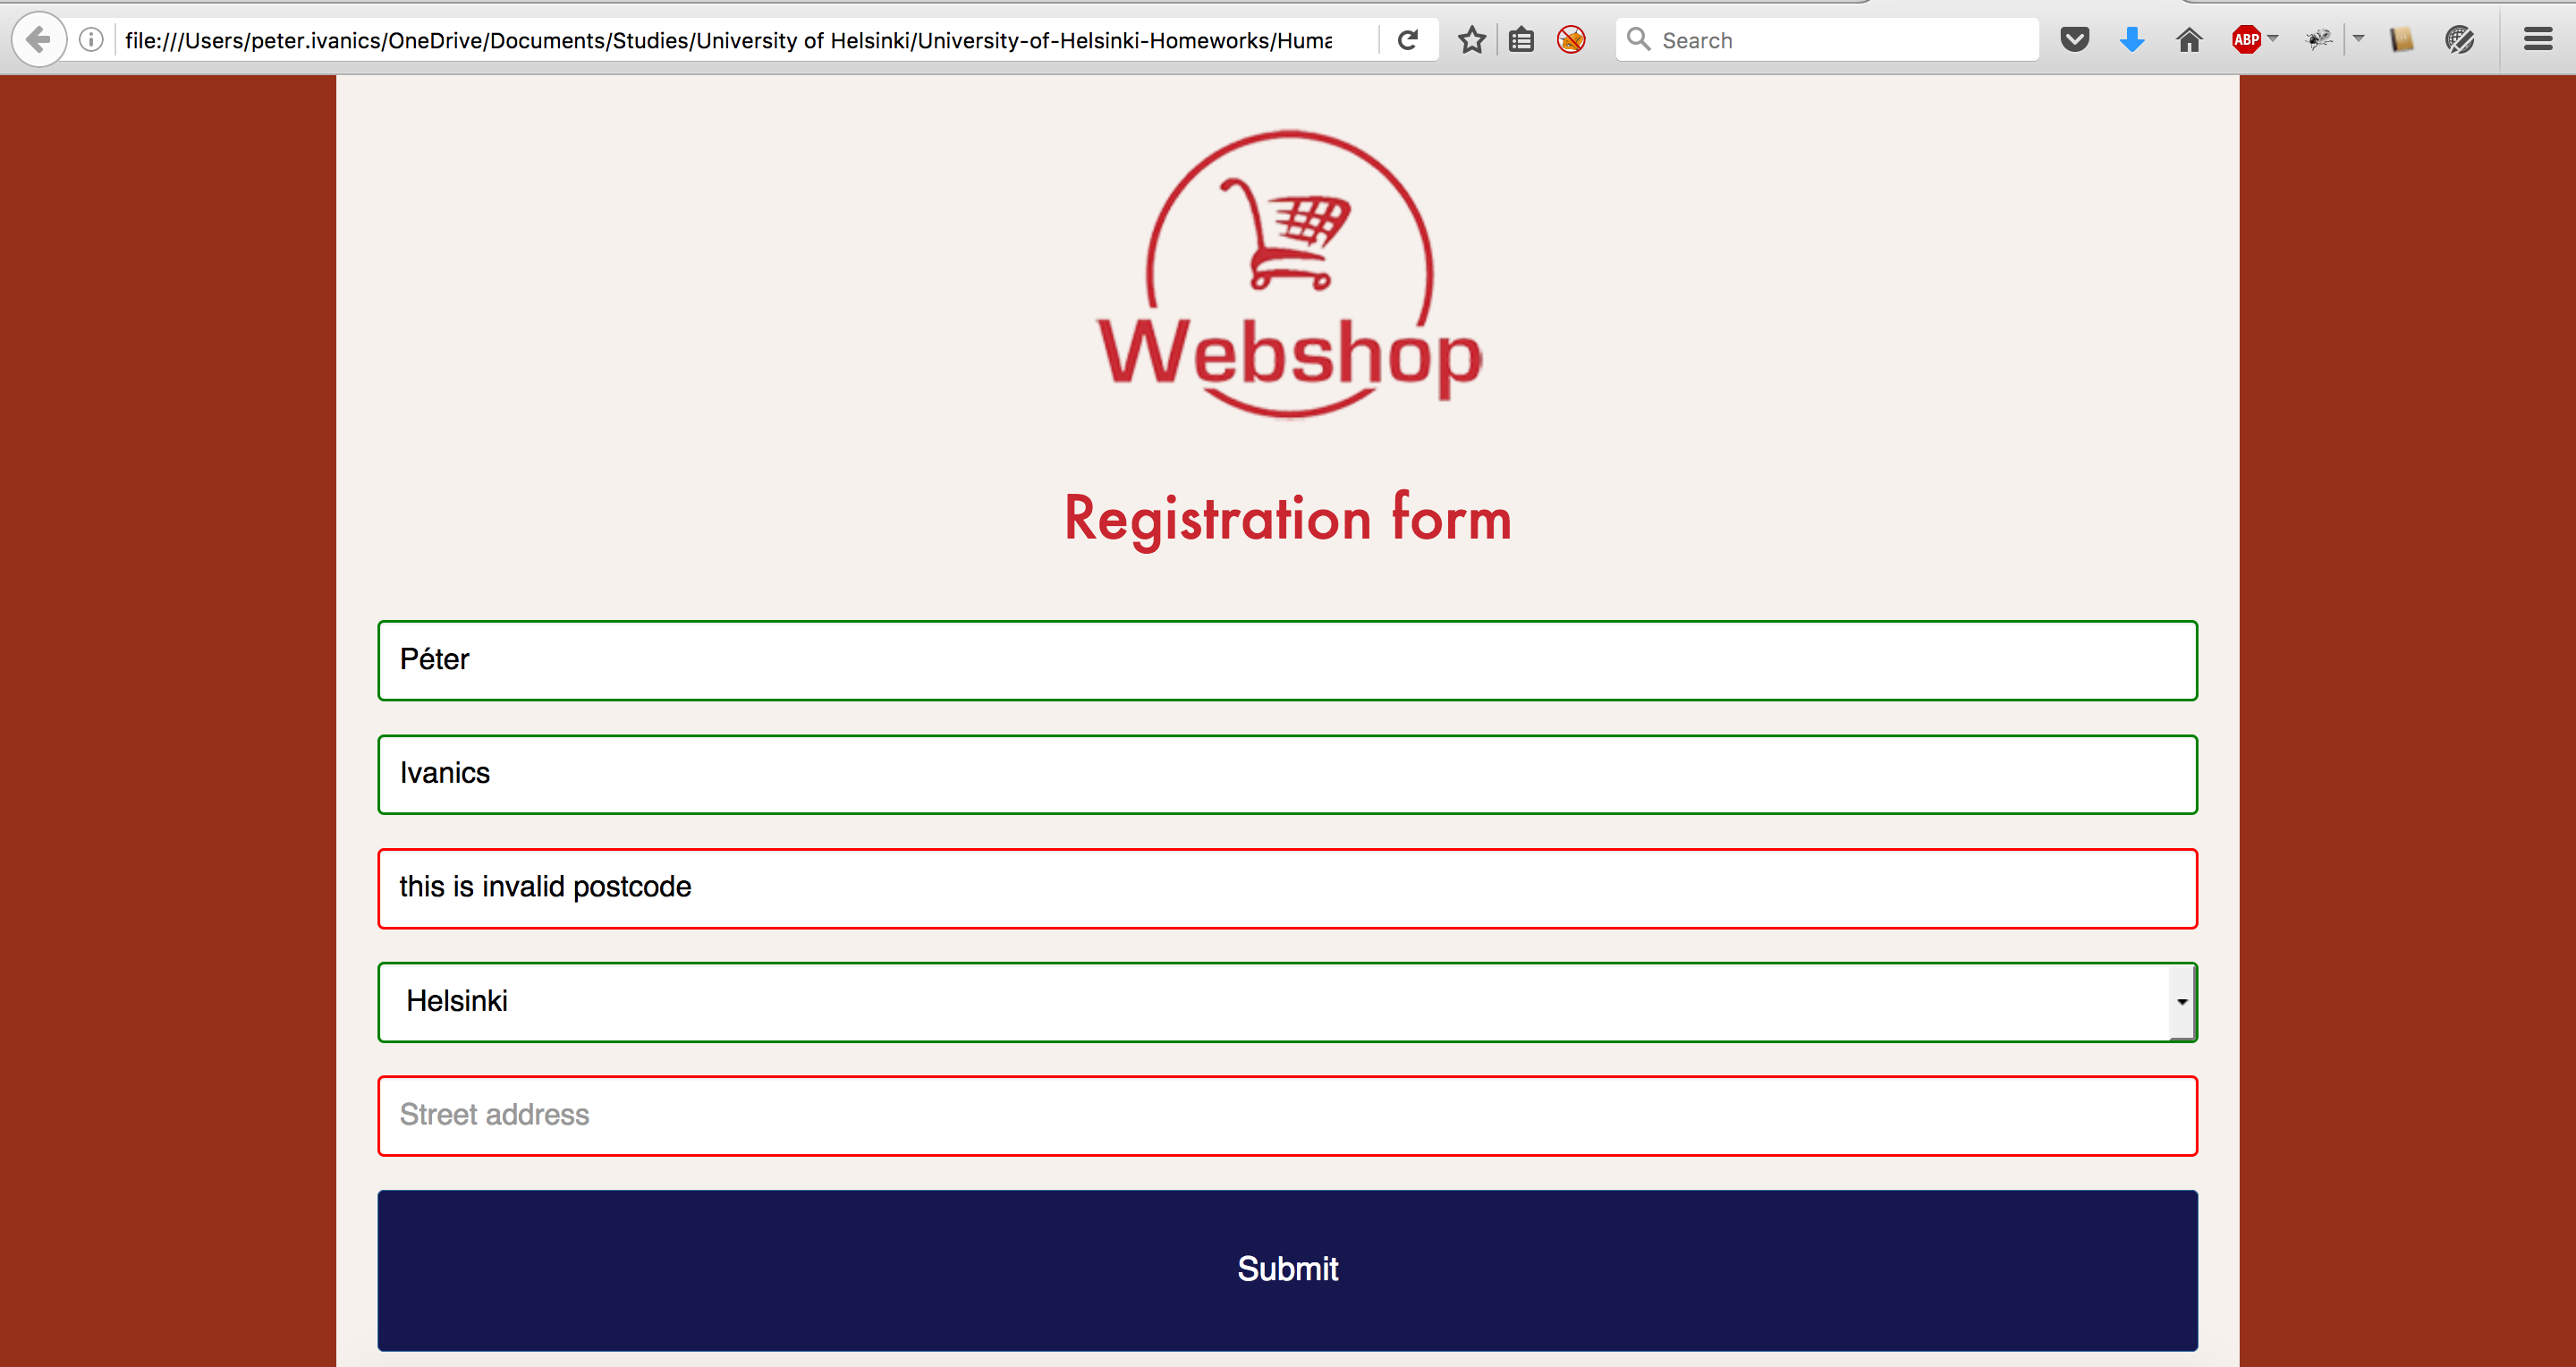
\includegraphics[height=0.4\textwidth]{images/final_webpage.png}
			\caption{The improved webpage right after opening.}
			\label{improved_webpage}
		\end{center}
	\end{figure}

\section{Unimplemented features}
	% [describe here the solutions that your web site does not have but which would be useful and important]
	Due to the short time-frame, only a subset of the proposals were implemented. To further increase usability, the following features/improvements should be addressed: 
	
	\begin{itemize}
		\item validating and sending the form upon the Submit button is pressed,
		\item displaying meaningful error messages pointing at the problematic text fields, e.g. "The postal code can contain only numerical characters", 
		\item confirmation screen after a successful registration, 
		\item auto-complete for the street address as the user is typing,
		\item selecting street address from a map.
	\end{itemize}
	
\pagebreak
\nocite{*}
\bibliographystyle{tktl}
\bibliography{bibliography}

\lastpage

\appendices

\pagestyle{empty}

%\internalappendix{1}{Model ABC}
%
%The appendices here are just models of the table of contents and the presentation. Each appendix 
%usually starts on its own page, with the name and number of the appendix at the top. Each appendix is paginated separately.
%
%In addition to complementing the main document, each appendix is also its own, independent entity. 
%This means that an appendix cannot be just an image or a piece of programming, but the appendix must explain its contents and meaning.

\end{document}


